\documentclass[11pt]{article}
\usepackage[a4paper,margin=19mm]{geometry}
\usepackage{fontspec}
\setmainfont{lmroman10-regular.otf}
\usepackage{amsmath,amssymb,amsthm,mathtools,amscd,xcolor,graphicx,hyperref}
\hypersetup{hidelinks}
\numberwithin{equation}{section}
\newtheorem{theorem}{Theorem}[section]
\newtheorem{lemma}[theorem]{Lemma}
\newtheorem{proposition}[theorem]{Proposition}
\newtheorem{corollary}[theorem]{Corollary}
\newtheorem{claim}[theorem]{Claim}
\newtheorem{fact}[theorem]{Fact}
\newtheorem{conjecture}[theorem]{Conjecture}
\theoremstyle{definition}
\newtheorem{definition}[theorem]{Definition}
\newtheorem{example}[theorem]{Example}
\newtheorem{remark}[theorem]{Remark}
\newtheorem{question}[theorem]{Question}
\theoremstyle{plain}
\newcommand{\C}{\mathbb C}
\newcommand{\R}{\mathbb R}
\newcommand{\Q}{\mathbb Q}
\newcommand{\Z}{\mathbb Z}
\newcommand{\N}{\mathbb N}
\newcommand{\eee}{\mathrm e}
\newcommand{\cclass}[1]{\textsf{#1}}
\newcommand{\cproblem}[1]{\textsc{#1}}
\newcommand{\ie}{i.\,e.}
\newcommand{\Ie}{I.\,e.}
\newcommand{\eg}{e.\,g.}
\newcommand{\Eg}{E.\,g.}
\newcommand{\phd}{Ph.\,D.}
\newcommand{\msc}{M.\,S.}
\newcommand{\bsc}{B.\,S.}
\newcommand{\expref}[2]{\hyperref[#2]{#1~\ref{#2}}}
\newcommand{\expeqref}[2]{\hyperref[#2]{#1~\eqref{#2}}}
\newcommand{\exprefsilent}[2]{\hyperref[#2]{#1}}
\providecommand{\etal}{et~al.}
\usepackage{eprint}
\usepackage{booktabs}
\usepackage{hyperref}
\usepackage{tabularx}
%
%
%
\usepackage{tikz}

%
%
%

\renewcommand{\geq}{\geqslant}
\renewcommand{\leq}{\leqslant}
\renewcommand{\ge}{\geq}
\renewcommand{\le}{\leq}

\newcommand{\union}{\mathbin{\cup}}
\newcommand{\intersect}{\mathbin{\cap}}

\newcommand{\tbd}[1]{\textcolor{red}{TBD: #1}}
\newcommand{\abs}[1]{\ensuremath\left|#1\right|}
\newcommand{\ceil}[1]{\ensuremath\left\lceil#1\right\rceil}
\newcommand{\set}[2]{\ensuremath{\left\{#1 \mid #2\right\}}}
\newcommand{\os}[1]{\ensuremath{\left\{#1\right\}}}
\newcommand{\bigO}{\mathcal{O}}

\newcommand{\FOLL}{\ensuremath{\mathsf{FOLL}}}
\newcommand{\AC}{\ensuremath{\mathsf{AC}}}
\newcommand{\ACC}{\ensuremath{\mathsf{ACC}}}
\newcommand{\qAC}{\ensuremath{\mathsf{qAC}}}
\newcommand{\TC}{\ensuremath{\mathsf{TC}}}
\newcommand{\NC}{\ensuremath{\mathsf{NC}}}
\newcommand{\PTIME}{\ensuremath{\mathsf{P}}}
%
\newcommand{\LOGSPACE}{\ensuremath{\mathsf{Logspace}}}
\newcommand{\NL}{\ensuremath{\mathsf{NL}}}
\newcommand{\NP}{\ensuremath{\mathsf{NP}}}
\newcommand{\Ppoly}{\ensuremath{\mathsf{P / poly}}}
\newcommand{\DPOLYLOGTIME}{\ensuremath{\mathsf{DPOLYLOGTIME}}}

\newcommand{\vC}{\mathbf{C}}
\newcommand{\vV}{\mathbf{V}}
\newcommand{\vW}{\mathbf{W}}
\newcommand{\vAb}{\mathbf{Ab}}
\newcommand{\vNil}{\mathbf{N}}
\newcommand{\vLI}{\mathbf{LI}}
\newcommand{\vCom}{\mathbf{Com}}
\newcommand{\vG}{\mathbf{G}}
\newcommand{\vRB}{\mathbf{RB}}

\newcommand{\GEN}{\ensuremath{\textsc{GEN}}}
\newcommand{\CSM}{\ensuremath{\textsc{CSM}}}
\newcommand{\Parity}{\ensuremath{\textsc{Parity}}}
\newcommand{\STCONN}{\ensuremath{\textsc{STConn}}}

\renewcommand{\C}{\ensuremath{\mathcal{C}}}

\newcommand{\SCGM}{Cayley groupoid membership}
\newcommand{\CCGM}{Cayley Groupoid Membership}
\newcommand{\SCSM}{Cayley semigroup membership}
\newcommand{\CCSM}{Cayley Semigroup Membership}
\newcommand{\SCGMP}{{\SCGM} problem}
\newcommand{\CCGMP}{{\CCGM} Problem}
\newcommand{\SCSMP}{{\SCSM} problem}
\newcommand{\CCSMP}{{\CCSM} Problem}
\newcommand{\SLPBP}{logarithmic power basis property}
\newcommand{\CLPBP}{Logarithmic Power Basis Property}
%
\newcommand{\SPLCP}{polylogarithmic circuits property}
%
\newcommand{\CPLCP}{Polylogarithmic Circuits Property}
%
%

\newcommand{\Hastad}{H{\aa}stad}
\newcommand{\Szemeredi}{Szemer{\'e}di}

\newcommand{\ms}{\hspace*{0.5pt}}

\makeatletter
\newcommand{\thickhline}{%
    \noalign {\ifnum 0=`}\fi \hrule height 1pt
    \futurelet \reserved@a \@xhline
}
\makeatother
\title{Logarithmic power bases give FOLL Cayley semigroup membership}
\author{Lukas Fleischer}
\date{doi:10.4086/toc.2022.v018a008; CC BY 3.0}
\begin{document}
\maketitle
\noindent\textit{Editorial note.} Complete original mathematical body149--1458 and original published bibliography retained. Original frontmatter/biography and native class remain in raw source/publication PDF assets. Existing article interface renders ToC notation for XeLaTeX only.\par\medskip
\noindent\textit{Editorial note.} One general subsemigroup-closed class FOLL theorem is counted. Earlier Barrington-Kadau-Lange-McKenzie strategy and quoted group results retain their original attribution. No novelty certification or mathematical review performed.\par\medskip
\noindent\textit{Editorial note.} Exact original CC BY3.0 retained. Authors own mathematics; no added assumptions, proof repair or independent certification.\par\medskip
\noindent\textit{Allowed standard prerequisites (editorial).}\begin{itemize}
\item Finite semigroups, circuit complexity and repeated squaring. Original closure and logarithmic power-basis assumptions retained, with cited earlier group algorithms and source-local Cayley circuit definitions.. Complete original width construction and recursive circuit implementation retained without replacing the general class theorem by a quoted group result.
\end{itemize}\medskip
\begin{abstract}
  The \emph{Cayley semigroup membership problem} asks, given a multiplication
  table representing a semigroup~$S$, a subset $X$ of $S$ and an element $t$ of
  $S$, whether $t$ can be expressed as a product of elements of $X$.
  %
  It is well-known that this problem is $\NL$-complete
  %
  %
%
%
under $\AC^0$-reductions.  %
  %
For groups, the problem can be solved in deterministic
 %
$\LOGSPACE$.   %
This raised the question of determining the exact complexity of this variant.
  %
  Barrington, Kadau, Lange and McKenzie showed that for Abelian groups and for
  certain solvable groups, the problem is contained in the complexity class
  $\FOLL$  %
  (polynomial-size, $O(\log\log n)$-depth circuits) %
  and they concluded that these variants are not hard,
  under $\AC^0$ reductions,  %
  for any complexity class containing the $\Parity$ language. The more
  general case of arbitrary groups remained open.
  %
  In this %
  article,  %
  we apply results by Babai and Szemer\'edi directly to this
  setting to show that the problem is solvable in $\qAC^0$ (quasi-polynomial
  size circuits of constant depth with unbounded fan-in). We prove a similar
  result for commutative semigroups. Combined with the Yao--\Hastad\
  %
  circuit lower bound,  %
  it follows immediately that {\SCSM} for groups and {\SCSM} for
  commutative semigroups are not hard,
  under $\AC^0$ reductions, %
  for any class containing $\Parity$.
  %
  Moreover, we prove that $\NL$-completeness already holds for the classes
  of $0$-simple semigroups and nilpotent semigroups.
  %
  Together with our results on groups and commutative semigroups, we prove the
  existence of a natural class of finite semigroups that generates a variety of
  finite semigroups with $\NL$-complete {\SCSM}, while the {\SCSMP} for the
  class itself is not $\NL$-hard.
  %
  We also discuss applications of our technique to $\FOLL$ and describe
  varieties for which the {\SCSMP} is in $\AC^0$.
\end{abstract}

\section{Introduction}

Back in 1976, Jones and Laaser studied the complexity of the \emph{generation
problem} which is formally defined as follows.
\vspace{1em}

\noindent
\begin{tabularx}{\textwidth}{p{1.25cm}X}
  \thickhline
  $\GEN$ \\
  \hline
  \textsf{Input}: & A set $G$, a binary operation $\circ \colon G \times G \to G$, a set $X \subseteq G$ and an element $t \in G$ \\
  \textsf{Question}: & Is $t$ contained in the smallest
  %
superset   %
of $X$ closed under $\circ$? \\
  \hline
\end{tabularx}
\vspace{1ex}

They showed that this problem is $\PTIME$-complete%
%
%
%
%
\footnote{In this paper, all completeness/hardness statements
are with respect to $\AC^0$ reductions.  Even though some of the
cited articles only claim completeness under $\LOGSPACE$ or $\NC^1$
reductions, their reductions can in fact be implemented in $\AC^0$.} %
\cite{JonesL76}, an observation which has since been used in many 
other $\PTIME$-completeness results.
%
Barrington and McKenzie later studied natural subproblems and connected them to
standard subclasses of $\PTIME$~\cite{BarringtonM91}.
%
Following~\cite{BarringtonKLM01}, the generation problem is also referred to as
\emph{\SCGMP}.
%
This terminology stems from the fact that the set $G$ forms a groupoid when
equipped with the operation $\circ$ and the objective is to decide whether $t$
belongs to the subgroupoid generated by $X$.
%
The prefix \emph{Cayley} is due to the representation of finite groupoid by its
multiplication table, often also called \emph{Cayley table}.

It is not surprising that imposing further structural properties on the
multiplication table affects the complexity of the {\SCGMP}.
%
For example, if the multiplication table is required to be associative, one
obtains the \emph{associative generation problem}, henceforth referred to as
\emph{\SCSMP}.
%
This decision problem is $\NL$-complete~\cite{JonesLL76}.
%
We will analyze its complexity when further restricting the semigroups encoded
by the input.
%
For a class of finite semigroups $\vC$, the \emph{{\SCSMP} for~$\vC$} is
defined as follows.
\vspace{1em}

\noindent
\begin{tabularx}{\textwidth}{p{1.25cm}X}
  \thickhline
  $\CSM(\vC)$ \\
  \hline
  \textsf{Input}: & The Cayley table of a semigroup $S \in \vC$, a set $X \subseteq S$ and an element $t \in S$ \\
  \textsf{Question}: & Is $t$ in the subsemigroup of $S$ generated by $X$? \\
  \hline
\end{tabularx}
\vspace{1ex}

The motivation for investigating this problem is two-fold.
%
%
First,   %
there is a direct connection between the {\SCSMP} and decision
problems for regular languages: a language $L \subseteq \Sigma^+$ is regular
if and only if there exist a finite semigroup~$S$, a morphism $\varphi \colon
\Sigma^+ \to S$ and a set $P \subseteq S$ such that $L = \varphi^{-1}(P)$.
%
Thus, morphisms to finite semigroups can be seen as a way of encoding regular
languages. For encoding such a semigroup, specifying the multiplication table
is a natural choice.
%
Deciding emptiness of a regular language represented by a morphism $\varphi
\colon \Sigma^+ \to S$ to a finite semigroup $S$ and a set $P \subseteq S$
boils down to checking whether any of the elements from the set $P$ is
contained in the subsemigroup of $S$ generated by the images of the letters of
$\Sigma$ under $\varphi$.
%
Conversely, the {\SCSMP} is a special case of the emptiness problem for regular
languages: an element $t \in S$ is contained in the subsemigroup generated by a
set $X \subseteq S$ if and only if the language $\varphi^{-1}(P)$ with $\varphi
\colon X^+ \to S, x \mapsto x$ and $P = \os{t}$ is non-empty.

%
Second,  %
we hope to get a better understanding of the connection between
algebra and low-level complexity classes included in $\NL$ in a fashion 
similar to the results of~\cite{BarringtonM91}.
%
In the past, several intriguing links between so-called \emph{varieties
of finite semigroups} and the computational complexity of algebraic problems
for such varieties were made.
%
For example, the word problem for a fixed finite semigroup was shown to be in
$\AC^0$ if the semigroup is aperiodic, in $\ACC^0$ if the semigroup is solvable
and $\NC^1$-complete otherwise~\cite{Barrington89,bt88jacm}.

\subparagraph{Related work.}

%
The first %
completeness results for the {\SCGMP} appeared in work by Jones and
Laaser~\cite{JonesL76}, and completeness results on the {\SCSMP} appeared in a
paper by Jones, Lien and Laaser~\cite{JonesLL76}.

The semigroup membership problem and its restrictions to varieties of finite
semigroups was also studied for other encodings of the input, such as matrix
semigroups~\cite{Babai85,BabaiS84,BabaiBIL96} or transformation
semigroups~\cite{Sims1967,FurstHopcroftLuks80,BabaiLS87,Beaudry88,BeaudryMT92,Beaudry94,Beaudry88thesis}.
%
In \cite{BabaiS84}, Babai and Szemer\'edi introduced the Black Box Group model,
and applied it to matrix groups over finite fields. The Black Box Group model
also has direct applications in the Cayley table model\,---\,however, to the
best of our knowledge, this connection has not been investigated prior to the
present paper.

Further systematic study of the group membership problem in the Cayley model
($\CSM(\vG)$, using our notation) began with a paper by Barrington and McKenzie
in 1991~\cite{BarringtonM91}.
%
They observed that the problem is in %
$\mathsf{SymmetricLogspace}$  %
which has been shown 
by Reingold in 2008~\cite{Reingold08} %
to be the same as deterministic %
$\LOGSPACE$,
%
and
they  %
suggested it might be complete for deterministic %
$\LOGSPACE$.
However, all attempts to obtain a hardness proof failed (in fact,
the conjecture is shown to be false in this %
paper).  %
%
There was no progress in a long time until Barrington, Kadau, Lange and
McKenzie showed  %
in 2001~\cite{BarringtonKLM01}  %
that for Abelian groups and certain solvable groups, the
problem lies in the complexity class $\FOLL$ %
(decidable by circuits of polynomial size and $O(\log\log n)$ depth) %
and thus cannot be hard for any
complexity class containing $\Parity$. 
%

The case of arbitrary finite groups remained open partly due to the lack of
awareness of the relevance of the early work by Babai and
Szemer\'edi~\cite{BabaiS84}.  %
With this paper we are closing this information gap. We give more
details of the connection in \expref{Section}{sec:parallel-alg}.

\subparagraph{Our contributions.}  %
%

We show that the {\SCSMP} for the variety
%
$\vG$ of finite groups   %
and the variety 
%
$\vCom$ of commutative semigroups %
%
are   %
contained in $\qAC^0$ and thus
cannot be hard for any class containing $\Parity$.
%
Our approach heavily relies on the application of techniques
from~\cite{BabaiS84} to the Cayley table setting.
%
The key observation is that every element of a group $G$
%
(or commutative    %
semigroup~$S$) can be computed by an algebraic circuit of size
$\mathcal{O}(\log^3 \abs{G})$  
%
(size $\mathcal{O}(\log^2 \abs{S})$, resp.)  %
over any set of generators.

By means of a closer analysis of the technique used by Jones, Lien and Laaser
in~\cite{JonesLL76}, we also show that the {\SCSMP} remains $\NL$-complete when
restricting the input to $0$-simple semigroups or to nilpotent semigroups.

Combining our results, we obtain that the {\SCSMP} for the class
$\vG \union \vCom$ 
is decidable in $\qAC^0$ (and thus not $\NL$-hard) while the {\SCSMP}
for the minimal variety of finite semigroups containing $\vG \union \vCom$ is
$\NL$-complete.

We discuss the extent to which our approach can be used to establish
membership of {\SCSM} variants %
in  %
the complexity class $\FOLL$.
%
Here, we use an idea based on repeated squaring. This technique generalizes
some of the main concepts used in~\cite{BarringtonKLM01}.
%
Finally, we give examples of varieties for which the {\SCSMP} is in $\AC^0$.

\section{Preliminaries}
\label{sec:prelim}

\subparagraph{Algebra.}

A semigroup $T$ is a \emph{subsemigroup} of $S$ if $T$ is a subset of $S$
closed under multiplication.
%
The \emph{direct product} of two semigroups $S$ and $T$ is the Cartesian
product $S \times T$ equipped with componentwise multiplication.
%
A semigroup $T$ is a \emph{quotient} of a semigroup $S$ if there exists a
surjective morphism $\varphi \colon S \to T$.
%
A semigroup $T$ \emph{divides} a semigroup $S$ if there exists a surjective
morphism from a subsemigroup of $S$ onto $T$.

For every element $s$ of a finite semigroup $S$, there exist natural
numbers $i, p > 0$ such that $s^{i+p} = s^i$.
%
This implies $s^{j+p} = s^j$ for all $j \ge i$. In particular, we have
$(s^{ip})^2 = s^{ip + ip} = s^{ip}$, which shows that in a finite semigroup,
every element has an idempotent power.
%
An element $z \in S$ is a \emph{zero element} if $sz = z = zs$ for all $s \in
S$. It is easy to see that every semigroup contains at most one zero element.
It is usually denoted by $0$.

A \emph{variety of finite semigroups} is a class of finite semigroups that is
closed under finite direct products and under taking divisors.
%
Since we are only interested in finite semigroups, we will henceforth use the
term \emph{variety} for a variety of finite semigroups.
%
Note that in the literature, such classes of semigroups are often called
\emph{pseudovarieties}, as opposed to Birkhoff varieties which are also closed
under infinite direct products.
%
The following varieties play an important role in this paper:
%
\begin{itemize}
  \item $\vAb$, the class of all finite Abelian groups,
  \item $\vCom$, the class of all finite commutative semigroups,
  \item $\vG$, the class of all finite groups,
  \item $\vNil$, the class of all finite \emph{nilpotent} semigroups, \ie, finite
    semigroups $S$ with a zero element~$0$ such that for all $s \in S$, there
    exists an integer $e \in \N$ with $s^e = 0$,
  \item $\vLI$, the class of all finite \emph{locally trivial} semigroups, \ie,
    finite semigroups $S$ where $ese = e$ for all elements $s \in S$ and all
    idempotent elements $e \in S$,
  \item $\vLI_k$, the class of all finite semigroups $S$ that satisfy $x_1
    \cdots x_k z y_k \cdots y_1 = x_1 \cdots x_k y_k \cdots y_1$ for all $x_1,
    \dots, x_k, y_1, \dots, y_k, z \in S$.
\end{itemize}
%
Note that by definition, the only idempotent element of a nilpotent semigroup
is the zero element.
%
For finite semigroups, having exactly one idempotent element which is a zero
element actually characterizes nilpotency:
%
for a finite semigroup $S$ with this property and an element $s \in S$,
choosing $e \in \N$ such that $s^e$ is idempotent, we obtain $s^e = 0$.
%
{}From this observation, it follows immediately that every finite nilpotent
semigroup is locally trivial, \ie, $\vNil \subseteq \vLI$.
%

It is easy to verify that every semigroup in $\vLI_k$ is locally trivial.
Moreover, if $S$ is a finite locally trivial semigroup, then $S$ belongs to
$\vLI_{\abs{S}}$. Therefore, $\vLI = \bigcup_{k \in \N} \vLI_k$. The classes
$\vLI_k$ form an infinite strict hierarchy within $\vLI$.

The \emph{join} of two varieties $\vV$ and $\vW$, denoted by $\vV \lor \vW$, is
the smallest variety containing both $\vV$ and $\vW$.
%
A semigroup $S$ is \emph{$0$-simple} if it contains a zero element $0$ and if
for each $s \in S \setminus \os{0}$, one has $SsS = S$.
%
The class of finite $0$-simple semigroups does not form a variety.

For a comprehensive introduction to the algebraic concepts used in this paper,
we refer to the textbooks~\cite{Howie95} and~\cite{pin86}.

\subparagraph{Complexity.}

We assume familiarity with standard definitions from circuit complexity;
see, \eg, %
\cite{Vollmer99} for an introduction.
%
We consider \emph{unbounded fan-in Boolean circuits} which consist of unbounded
fan-in AND gates, unbounded fan-in OR gates and fan-in-1 NOT gates.
%
The \emph{size} of such a circuit is the total number of AND and OR gates.
%
The \emph{length} of a path in the circuit is the total number of AND and OR
gates occurring on the path.
%
The length of the longest path from an input gate to the output gate is the
\emph{depth} of the circuit.
%
Note that NOT gates are not counted when measuring the size or depth of a
circuit.
%
A function has \emph{quasi-polynomial} growth if it is contained in
$2^{\bigO(\log^c n)}$ for some fixed $c \in \N$.

Throughout the paper, we will consider the following unbounded fan-in Boolean
circuit families:
%
\begin{itemize}
  \item $\AC^0$, languages decidable by circuit families of depth $\bigO(1)$
    and polynomial size,
  \item $\qAC^0$, languages decidable by circuit families of depth $\bigO(1)$
    and quasi-polynomial size,
  \item $\FOLL$, languages decidable by circuit families of depth
    $\bigO(\log \log n)$ and polynomial size,
  \item $\AC^1$, languages decidable by circuit families of depth
    $\bigO(\log n)$ and polynomial size,
  \item $\Ppoly$, languages decidable by circuit families of polynomial size
    (and unbounded depth).
\end{itemize}

We will also briefly refer to the complexity classes $\ACC^0$, $\TC^0$,
$\NC^1$, $\LOGSPACE$ and $\NL$.
%
It is known that the \Parity~function cannot be computed by $\AC^0$, $\FOLL$ or
$\qAC^0$ circuits. This follows directly from H{\aa}stad's and Yao's famous
lower bound results~\cite{Hastad86,Yao85}, which state that the number of
Boolean gates required for a depth-$d$ circuit to compute $\Parity$ is
exponential in $n^{1/(d-1)}$.

\begin{remark}
  We use $\AC^0$, $\ACC^0$, $\TC^0$, $\NC^1$, $\AC^1$, $\qAC^0$, $\FOLL$ to
  refer to the \emph{non-uniform} variants of these complexity classes, even
  though the same identifiers are sometimes also used to refer to uniform
  variants in related work.
  %
  While our proofs also work in the uniform setting, our main results do not
  require uniformity.
  %
  Proving that our algorithms can also be implemented as uniform circuits
  requires introducing the non-standard notion of $\DPOLYLOGTIME$-uniformity
  and some caution in the proofs. To avoid additional technical details and to
  keep the proofs short and self-contained, we refrain from doing so.
  %
  \label{}
\end{remark}

\section{Hardness results}

Before looking at parallel algorithms for the {\SCSMP}, we establish two new
$\NL$-hardness results.
%
To this end, we first analyze the construction already used by Jones, Lien and
Laaser~\cite{JonesLL76}.
%
It turns out that the semigroups used in their reductions are $0$-simple which
leads to the following result.

\begin{theorem}
  For a class containing all $0$-simple semigroups, the {\SCSMP} is
  $\NL$-complete (under $\AC^0$ many-one reductions).
  \label{thm:0-simple}
\end{theorem}

\begin{proof}
  To keep the proof self-contained, we briefly describe the reduction from
  the connectivity problem for directed graphs (henceforth called $\STCONN$) to
  the {\SCSMP} given in~\cite{JonesLL76}.

  Let $G = (V, E)$ be a directed graph.
  %
  We construct a semigroup on the set $S = V \times V \union \os{0}$ where $0$
  is a zero element and the multiplication rule for the remaining elements is
  %
  \begin{equation*}
    (v, w) \cdot (x, y) =
    \begin{cases}
      (v, y) & \text{if $w = x$}, \\
      0 & \text{otherwise}.
    \end{cases}
  \end{equation*}
  %
  By construction, the subsemigroup of $S$ generated by $E \union \set{(v,
  v)}{v \in V}$ contains an element $(s, t)$ if and only if $t$ is reachable
  from $s$ in $G$.
  %
  To see that the semigroup $S$ is $0$-simple, note that for pairs of arbitrary
  elements $(v, w) \in V \times V$ and $(x, y) \in V \times V$, one has $(x, v)
  (v, w) (w, y) = (x, y)$, which implies $S (v, w) S = S$.
\end{proof}

In order to prove $\NL$-completeness for another common class of semigroups, we
use a construction reminiscent of the ``layer technique'', which is usually
used to show that $\STCONN$ remains $\NL$-complete when the inputs are acyclic
graphs.

\begin{theorem}
  $\CSM(\vNil)$ is $\NL$-complete (under $\AC^0$ many-one reductions).
  \label{thm:nil}
\end{theorem}

\begin{proof}
  Following the proof of \expref{Theorem}{thm:0-simple}, we describe an $\AC^0$
  reduction of $\STCONN$ to $\CSM(\vNil)$.

  Let $G = (V, E)$ be a directed graph with $n$ vertices.
  %
  We construct a semigroup on the set $S = V \times \os{1, \dots, n-1} \times V
  \union \os{0}$ where $0$ is a zero element and the multiplication rule for
  the remaining elements is
  %
  \begin{equation*}
    (v, i, w) \cdot (x, j, y) =
    \begin{cases}
      (v, i + j, y) & \text{if $w = x$ and $i + j < n$}, \\
      0 & \text{otherwise}.
    \end{cases}
  \end{equation*}
  %
  The subsemigroup of $S$ generated by the set $\set{(v, 1, w)}{v = w
  \text{~or~} (v, w) \in E}$ contains the element $(s, n-1, t)$ if and only if
  $t$ is reachable (in less than $n$ steps) from $s$ in $G$.
  %
  Clearly, the zero element is the only idempotent in $S$, so $S$ is nilpotent.
  %
  Also, it is readily verified that the reduction can be performed by an
  $\AC^0$ circuit family.
\end{proof}

%
\section{Parallel algorithms for {\SCSM}}  %
\label{sec:parallel-alg}

In the Black Box Group model introduced by Babai and
\Szemeredi~\cite{BabaiS84}, %
group elements  %
are encoded by
%
bit strings of uniform length,  %
and group
operations (computing products and inverse elements%
%
\footnote{Babai and \Szemeredi~\cite{BabaiS84} consider the more general
model where multiple strings may encode the same group
element; in this case, an oracle to recognize the identity
element needs to be added.  However, in the present paper we only
consider the case of unique encoding.})  %
are performed by an
oracle. Babai and \Szemeredi\ showed that subgroup membership
is in $\NP$ relative to the group oracle.
%
Together with the following observations, it follows that in the Cayley table
setting, subgroup membership can be decided in non-deterministic
polylogarithmic time in the random-access Turing machine model:
%
\begin{itemize}
  \item Without loss of generality, we can assume that there are only
    logarithmically many generators in the input, since a generating subset
    of this size can be guessed in non-deterministic polylogarithmic time.
    
  \item A single oracle query can be simulated in non-deterministic logarithmic
    time (non-determinism is only required to compute the inverse of an
    element).
\end{itemize}
%
Since $\qAC^0$ contains all languages decidable in non-deterministic
polylogarithmic time, it follows that $\CSM(\vG)$ is in $\qAC^0$.

In the remainder of this section, we will give a more self-contained proof of
this result, and expand it to other classes of semigroups.
%
We will use algebraic circuits as a succinct representation of elements in an
algebraic structure, %
similarly  %
to the approach taken in~\cite{BabaiS84}.
%
Unlike in usual algebraic circuits, in the context of the {\SCSMP}, the
algebraic structure is not fixed but given as part of the input.
%
We will introduce so-called Cayley circuits to deal with this setting.
%
Since these circuits will be used for the {\SCSMP} only, we confine ourselves
to cases where the algebraic structure is a finite semigroup.

\subsection{Cayley circuits}

A \emph{Cayley circuit} is a directed acyclic graph with topologically ordered
vertices such that each vertex has in-degree $0$ or $2$.
%
In the following, to avoid technical subtleties when squaring an element, we
allow multi-edges.
%
The vertices of a Cayley circuit are called \emph{gates}. The vertices with
in-degree $0$ are called \emph{input gates} and vertices with in-degree $2$ are
called \emph{product gates}. Each Cayley circuit also has a designated gate of
out-degree $0$, called the \emph{output gate}. For simplicity, we assume that
the output gate always corresponds to the maximal gate with regard to the
vertex order.
%
The \emph{size} of a Cayley circuit $\C$, denoted by $\abs{\C}$, is the number
of gates of $\C$.
%
An \emph{input} to a Cayley circuit $\C$ with $k$ input gates consists of a
finite semigroup $S$ and elements $x_1, \dots, x_k$ of $S$.
%
Given such an input, the \emph{value} of the $i$-th input gate is $x_i$ and the
value of a product gate, whose predecessors have values $x$ and $y$, is the
product $x \cdot y$ in $S$. The \emph{value of the circuit $\C$} is the value
of its output gate.
%
We will denote the value of $\C$ under a finite semigroup $S$ and elements
$x_1, \dots, x_k \in S$ by $\C(S, x_1, \dots, x_k)$.

A Cayley circuit can be seen as a circuit in the usual sense: the finite
semigroup $S$ and the input gate values are given as part of the input and the
functions computed by product gates map a tuple, consisting of semigroup $S$
and two elements of $S$, to another element of $S$.
%
We say that a Cayley circuit with $k$ input gates can be \emph{simulated} by a
family of unbounded fan-in Boolean circuits $(\C_n)_{n \in \N}$ if, given the
encodings of a finite semigroup $S$ and of elements $x_1, \dots, x_k$ of $S$ of
total length $n$, the circuit $\C_n$ computes the encoding of $\C(S, x_1,
\dots, x_k)$.
%
For a semigroup $S$ with $N$ elements, we assume that the elements of $S$ are
encoded by the integers $\os{0, \dots, N-1}$ such that the encoding of a single
element uses $\ceil{\log N}$ bits. The semigroup itself is given as a
multiplication table with $N^2$ entries of $\ceil{\log N}$ bits each.

\begin{proposition}
  Let $\C$ be a Cayley circuit of size $m$.
  %
  Then, $\C$ can be simulated by a family of unbounded fan Boolean circuits
  $(\C_n)_{n \in \N}$ of depth $2$ and size at most $n^m$.
  %
  \label{prop:simulation}
\end{proposition}

\begin{proof}
  Let $\C$ be a Cayley circuit with $k$ input gates and $m-k$ product gates.
  %
  We want to construct a Boolean circuit that can be used for all finite
  semigroups $S$ with a fixed number of elements $N$.
  %
  The input to such a circuit consists of $n = (N^2 + k) \ceil{\log N}$ bits.

  For a fixed vector $(y_1, \dots, y_m) \in S^m$, one can check using a single
  AND~gate (and additional NOT~gates at some of the incoming wires) whether
  $(y_1, \dots, y_m)$ corresponds to the sequence of values occurring at the
  gates of $\C$ under the given inputs.
  %
  To this end, for each gate $i \in \os{1, \dots, m}$ of $\C$, we add
  $\ceil{\log N}$ incoming wires to this AND~gate:
  %
  if the $i$-th gate of $\C$ is an input gate, we feed the bits of the
  corresponding input value into the AND~gate, complementing the $j$-th bit if
  the $j$-th bit of $y_i$ is zero.
  %
  If the $i$-th gate is a product gate and has incoming wires from gates $\ell$
  and $r$, we connect the entry $(y_\ell, y_r)$ of the multiplication table to
  the AND~gate, again complementing bits corresponding to 0-bits of $y_i$.

  To obtain a Boolean circuit simulating $\C$, we put such AND~gates for all
  vectors of the form $(y_1, \dots, y_m) \in S^m$ in parallel. In a second
  layer, we create $\ceil{\log N}$ OR gates and connect the AND~gate for a
  vector $(y_1, \dots, y_m)$ to the $j$-th OR~gate if and only if the $j$-th
  bit of $y_m$ is one.
  %
  The idea is that exactly one of the AND~gates\,---\,the gate corresponding to
  the vector of correct guesses of the gate values of $\C$\,---\,evaluates
  to~$1$ and the corresponding output value $y_m$ then occurs as output value
  of the OR~gates.
  %
  This circuit has depth $2$ and size $N^m + \ceil{\log N} \le n^m$.
\end{proof}

%
\subsection{The {\SPLCP}}    %

When analyzing the complexity of $\CSM(\vAb)$, Barrington {\it et al.}
introduced the so-called \emph{\SLPBP}. A class of semigroups has the {\SLPBP}
if %
every set $X$ of generators  %
for a semigroup $S$ of cardinality $N$ from the
family has the property that every element of $S$ can be written as a product
of at most $\log(N)$ many powers of elements of $X$.
%
In~\cite{BarringtonKLM01}, it was shown that the class of Abelian groups has
the {\SLPBP}. Using a different technique, this result can easily be extended to
arbitrary commutative semigroups.

\begin{lemma}
  The variety $\vCom$ has the {\SLPBP}.
  \label{lem:com}
\end{lemma}
%
\begin{proof}
  Suppose that $S$ is a commutative semigroup of size $N$ and let $X$ be a set
  of generators for $S$.
  %
  Let $y \in S$ be an arbitrary element.
  %
  We choose $k \in \N$ to be the smallest value such that there exist elements
  $x_1, \dots, x_k \in X$ and integers $i_1, \dots, i_k \in \N$ with $y =
  x_1^{i_1} \cdots x_k^{i_k}$.
  %
  Assume, for the sake of contradiction, that $k > \log(N)$.

  The power set $\mathcal{P}(\os{1, \dots, k})$ forms a semigroup when equipped
  with set union as binary operation.
  %
  Consider the morphism $h \colon \mathcal{P}(\os{1, \dots, k}) \to S$ defined
  by $h(\os{j}) = x_j^{i_j}$ for all $j \in \os{1, \dots, k}$. This morphism is
  well-defined because $S$ is commutative.

  Since $\abs{\mathcal{P}(\os{1, \dots, k})} = 2^k > 2^{\log(N)} = \abs{S}$, we
  know by the pigeonhole principle that there exist two sets $K_1, K_2
  \subseteq \os{1, \dots, k}$ with $K_1 \ne K_2$ and $h(K_1) = h(K_2)$. We may
  assume, without loss of generality, that there exists some $j \in K_1
  \setminus K_2$.
  %
  Now, because
  %
  \begin{equation*}
    y = h(\os{1, \dots, k}) = h(K_1) \ms h(\os{1, \dots, k} \setminus K_1) = h(K_2) \ms h(\os{1, \dots, k} \setminus K_1)
  \end{equation*}
  %
  and since neither $K_2$ nor $\os{1, \dots, k} \setminus K_1$ contain $j$, we
  know that $y$ can be written as a product of powers of elements $x_i$ with $1
  \le i \le k$ and $i \ne j$, contradicting the choice of~$k$.
\end{proof}

For the analysis of arbitrary groups, we introduce a more general concept. It
is based on the idea that algebraic circuits (Cayley circuits with fixed
inputs) can be used for succinct representations of semigroup elements.

%
%
\begin{example}[repeated squaring]   %
  Let $e \in \N$ be a positive integer.
  %
  Then, one can construct a Cayley circuit of size at most $2\ceil{\log e}$
  which computes, given a finite semigroup $S$ and an element $x \in S$ as
  input, the power $x^e$ in $S$.
  %
  If $e = 1$, the circuit only consists of the input gate.
  %
  If $e$ is even, the circuit is obtained by taking the circuit for $e/2$,
  adding a product gate and creating two edges from the output gate of the
  circuit for $e/2$ to the new gate.
  %
  If $e$ is odd, the circuit is obtained by taking the circuit for $e-1$ and
  connecting it to a new product gate. In this case, the second incoming edge
  for the new gate comes from the input gate.
  %
  \label{ex:power}
\end{example}

%
A class of semigroups has the \emph{\SPLCP} if there exists a constant $c \in
\N$ such that for each semigroup $S$ of cardinality $N$ from the class, for
each subset $X$ of $S$ and for each $y$ in the subsemigroup generated by $X$,
there exists a Cayley circuit $\C$ of size $\log^c(N)$ with $k$ input gates and
there exist $x_1, \dots, x_k \in X$ such that $\C(S, x_1, \dots, x_k) = y$.

For classes closed under taking subsemigroups, such as varieties of finite
semigroups, this is equivalent to saying that each element $y$ of a semigroup
of cardinality $N$ can be represented by a Cayley circuit of size $\log^c(N)$
over any set of generators.
%
Alternatively, the {\SPLCP} can be defined in terms of \emph{straight-line
programs}; this connection will be used further below.

\begin{proposition}
  Let $\vC$ be a family of semigroups that is closed under subsemigroups and
  has the {\SLPBP}. Then $\vC$ has the {\SPLCP}.
  \label{prop:lpbp-plcp}
\end{proposition}
%
\begin{proof}
  Let $X$ be a subset of a semigroup $S$ of cardinality $N$. Let $y$ be in the
  subsemigroup generated by $X$.
  %
  Then, we have $y = x_1^{i_1} \cdots x_k^{i_k}$ for some $x_1, \dots, x_k \in
  X$  with $k \le \log(N)$ and $i_1, \dots, i_k \in \N$.
  %
  By the pigeonhole principle, we may assume without loss of generality that
  $1 \le i_1, \dots, i_k \le N$.
  %
  Using the method from \expref{Example}{ex:power}, one can construct Cayley
  circuits $\C_1, \dots, \C_k$ of size at most $2\ceil{\log N}$ such that
  $\C_j(S, x) = x^{i_j}$ for all $j \in \os{1, \dots, k}$ and $x \in S$. Using
  $k-1$ additional product gates $\mathcal{D}$, these circuits can be combined
  to a single circuit $\C$ with $\C(S, x_1, \dots, x_k) = x_1^{i_1} \cdots
  x_k^{i_k} = y$.
  %
  The construction is depicted in \expref{Figure}{fig:lpbp-plcp}.

  In total, the resulting circuit consists of $k \cdot 2\ceil{\log N} + k - 1 <
  5 \log^2(N)$ gates.
\end{proof}

\begin{figure}[t]
  \centering
  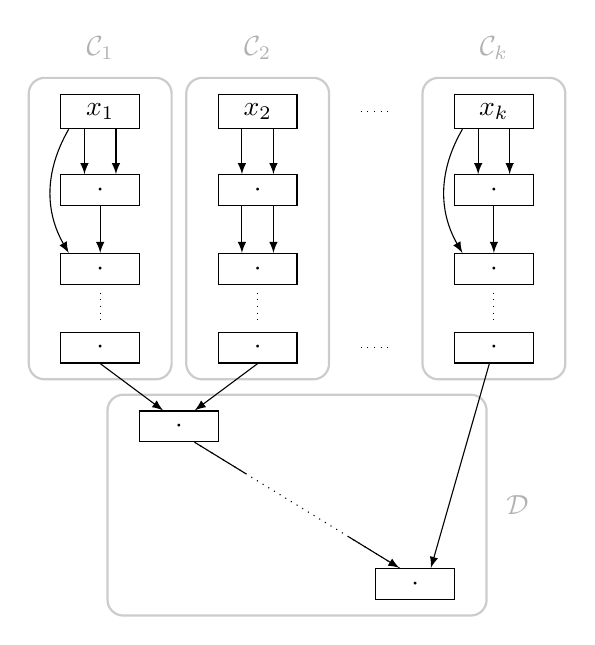
\begin{tikzpicture}[node distance=1cm]
    \node[draw,minimum width=1cm] (1-1) {$x_1$};
    \node[draw,minimum width=1cm] (1-2) [below of=1-1] {$\cdot$};
    \node[draw,minimum width=1cm] (1-3) [below of=1-2] {$\cdot$};
    \node[draw,minimum width=1cm] (1-4) [below of=1-3] {$\cdot$};

    \node[draw,minimum width=1cm] (2-1) [right of=1-1,xshift=1cm] {$x_2$};
    \node[draw,minimum width=1cm] (2-2) [below of=2-1] {$\cdot$};
    \node[draw,minimum width=1cm] (2-3) [below of=2-2] {$\cdot$};
    \node[draw,minimum width=1cm] (2-4) [below of=2-3] {$\cdot$};

    \node[draw,minimum width=1cm] (k-1) [right of=2-1,xshift=2cm] {$x_k$};
    \node[draw,minimum width=1cm] (k-2) [below of=k-1] {$\cdot$};
    \node[draw,minimum width=1cm] (k-3) [below of=k-2] {$\cdot$};
    \node[draw,minimum width=1cm] (k-4) [below of=k-3] {$\cdot$};

    \node[draw,minimum width=1cm] (a) [below of=1-4,xshift=1cm] {$\cdot$};
    \node[draw,minimum width=1cm] (c) [below of=k-4,xshift=-1cm,yshift=-2cm] {$\cdot$};

    \path[-latex] ([xshift=-2mm]1-1.south) edge ([xshift=-2mm]1-2.north);
    \path[-latex] ([xshift=+2mm]1-1.south) edge ([xshift=+2mm]1-2.north);
    \path[-latex] ([xshift=+0mm]1-2.south) edge ([xshift=+0mm]1-3.north);
    \path[-latex] ([xshift=-4mm]1-1.south) [bend right] edge ([xshift=-4mm]1-3.north);
    \path[dotted] ([yshift=-1mm]1-3.south) edge ([yshift=1mm]1-4.north);

    \path[-latex] ([xshift=-2mm]2-1.south) edge ([xshift=-2mm]2-2.north);
    \path[-latex] ([xshift=+2mm]2-1.south) edge ([xshift=+2mm]2-2.north);
    \path[-latex] ([xshift=-2mm]2-2.south) edge ([xshift=-2mm]2-3.north);
    \path[-latex] ([xshift=+2mm]2-2.south) edge ([xshift=+2mm]2-3.north);
    \path[dotted] ([yshift=-1mm]2-3.south) edge ([yshift=1mm]2-4.north);

    \path[-latex] ([xshift=-2mm]k-1.south) edge ([xshift=-2mm]k-2.north);
    \path[-latex] ([xshift=+2mm]k-1.south) edge ([xshift=+2mm]k-2.north);
    \path[-latex] ([xshift=+0mm]k-2.south) edge ([xshift=+0mm]k-3.north);
    \path[-latex] ([xshift=-4mm]k-1.south) [bend right] edge ([xshift=-4mm]k-3.north);
    \path[dotted] ([yshift=-1mm]k-3.south) edge ([yshift=1mm]k-4.north);

    \path[dotted] ([xshift=+8mm]2-1.east) edge ([xshift=-8mm]k-1.west);
    \path[dotted] ([xshift=+8mm]2-4.east) edge ([xshift=-8mm]k-4.west);

    \path[-latex] ([xshift=+0mm]1-4.south) edge ([xshift=-2mm]a.north);
    \path[-latex] ([xshift=+0mm]2-4.south) edge ([xshift=+2mm]a.north);
    \draw[dotted] ([xshift=+2mm]a.south) -- ([xshift=-2mm]c.north) coordinate[near start](x) coordinate[near end](y);
    \path[-] ([xshift=+2mm]a.south) edge (x);
    \path[-latex] (y) edge ([xshift=-2mm]c.north);
    \path[-latex] (k-4) edge ([xshift=+2mm]c.north);

    \draw[thick,opacity=.2,rounded corners=2mm] ([shift={(-4mm,+2mm)}]1-1.north west) rectangle ([shift={(+4mm,-2mm)}]1-4.south east);
    \node[draw=none,color=gray!60] (C1) [above of=1-1,yshift=-2mm] {$\C_1$};
    \draw[thick,opacity=.2,rounded corners=2mm] ([shift={(-4mm,+2mm)}]2-1.north west) rectangle ([shift={(+4mm,-2mm)}]2-4.south east);
    \node[draw=none,color=gray!60] (C2) [above of=2-1,yshift=-2mm] {$\C_2$};
    \draw[thick,opacity=.2,rounded corners=2mm] ([shift={(-4mm,+2mm)}]k-1.north west) rectangle ([shift={(+4mm,-2mm)}]k-4.south east);
    \node[draw=none,color=gray!60] (C3) [above of=k-1,yshift=-2mm] {$\C_k$};
    \draw[thick,opacity=.2,rounded corners=2mm] ([shift={(-4mm,+2mm)}]a.north west) rectangle ([shift={(+4mm,-2mm)}]c.south east);
    \node[draw=none,color=gray!60] (D) [right of=c,xshift=3mm,yshift=10mm] {$\mathcal{D}$};
  \end{tikzpicture}
  \caption{The Cayley circuit $\C$ from \expref{Proposition}{prop:lpbp-plcp}}
  \label{fig:lpbp-plcp}
\end{figure}

Let $G$ be a finite group and let $X$ be a subset of $G$. A sequence $(g_1,
\dots, g_\ell)$ of elements of $G$ is a \emph{straight-line program over $X$}
if for each $i \in \os{1, \dots, \ell}$, we have $g_i \in X$ or $g_i =
g_p^{-1}$ or $g_i = g_p g_q$ for some $p, q < i$.
%
The number $\ell$ is the \emph{length} of the straight-line program and the
elements of the sequence are said to be \emph{generated} by the straight-line
program.
%
The following result by Babai and Szemer\'edi~\cite{BabaiS84} is 
commonly known as the \emph{Reachability Lemma}.

\begin{lemma}[Reachability Lemma]
  Let $G$ be a finite group and let $X$ be a set of generators of $G$.
  %
  Then, for each element $t \in G$, there exists a straight-line program over
  $X$ generating $t$ which has length at most $(\log \abs{G} + 1)^2$.
  %
  \label{lem:reachability}
\end{lemma}

The proof of this lemma is based on a technique called ``cube doubling''. For
details, we refer to~\cite{Babai91}.
%
It is now easy to see that groups admit polylogarithmic circuits.

\begin{lemma}
  The variety $\vG$ has the {\SPLCP}.
  %
  \label{lem:groups}
\end{lemma}
%
\begin{proof}
  Let $G$ be a group of order $N$, let $X$ be a subset of $G$ and let $y$ be an
  element in the subgroup of $G$ generated by $X$.
  %
  By \expref{Lemma}{lem:reachability}, we know that there exists a straight-line
  program $(g_1, \dots, g_\ell)$ over $X$ with $\ell \le (\log(N) + 1)^2$ and
  $g_\ell = y$.
  %
  We may assume that the elements $g_1, \dots, g_\ell$ are pairwise distinct.
  %
  It suffices to describe how to convert this straight-line program into a
  Cayley circuit $\C$ and values $x_1, \dots, x_k \in X$ such that $\C(S, x_1,
  \dots, x_k) = y$.

  We start with an empty circuit and with $k = 0$ and process the elements of
  the straight-line program left to right. For each element $g_i$, we add gates
  to the circuit. The output gate of the circuit obtained after processing the
  element $g_i$ will be called the \emph{$g_i$-gate}.

  If the current element $g_i$ is contained in $X$, we increment $k$, add a new
  input gate to the circuit and let $x_k = g_i$.
  %
  If the current element $g_i$ can be written as a product $g_p g_q$ with
  $p, q < i$, we add a new product gate to the circuit and connect the
  $g_p$-gate as well as the $g_q$-gate to this new gate.
  %
  If the current element $g_i$ is an inverse $g_p^{-1}$ with $p < i$, we take a
  circuit $\C'$ with $2\ceil{\log N}$ gates and with $\C'(G, x) = x^{N-1}$ for
  all $x \in S$.
  %
  Such a circuit can be built by using the powering technique illustrated in
  \expref{Example}{ex:power}.
  %
  We add $\C'$ to $\C$, replacing its input gate
  by an edge coming from the $g_p$-gate.

  The resulting circuit has size at most $(\log(N) + 1)^2 \cdot 2\ceil{\log N}
  \le 2(\log(N) + 1)^3$.
\end{proof}

We will now show that for classes of semigroups with the {\SPLCP}, one can
solve the {\SCSMP} in $\qAC^0$.

\begin{theorem}
  Let $\vC$ be a class of semigroups with the {\SPLCP}.
  %
  Then $\CSM(\vC)$ is in $\qAC^0$.
  %
  \label{thm:qACzero}
\end{theorem}
%
\begin{proof}
  We construct a family of unbounded fan-in constant-depth Boolean circuits
  with quasi-polynomial size, deciding, given the multiplication table of a
  semigroup $S \in \vC$, a set $X \subseteq S$ and an element $t \in S$ as
  inputs, whether $t$ is in the subsemigroup generated by $X$.

  Since $\vC$ has the {\SPLCP}, we know that, for some constant $c \in \N$, the
  element $t$ is in the subsemigroup generated by $X$ if and only if there
  exist a Cayley circuit $\C$ of size $\log^c(n)$ and inputs $x_1, \dots, x_k
  \in X$ such that $\C(S, x_1, \dots, x_k) = t$.
  %
  There are at most $(\log^{c}(n) \cdot \log^{c}(n))^{\log^c(n)} = 2^{2c \ms
  \log^c(n) \log \log(n)}$ different Cayley circuits of this size.
  %
  Let us consider one of these Cayley circuits $\C$. Suppose that $\C$ has $k$
  input gates.
  %
  By \expref{Proposition}{prop:simulation}, there exists an unbounded fan-in
  constant-depth Boolean circuit of size $n^{\log^c n} = 2^{\log^{c+1} n}$
  deciding on input $S$ and elements $x_1, \dots, x_k \in S$ whether $\C(S,
  x_1, \dots, x_k) = t$.
  %
  There are at most $n^k \le n^{\log^c n} = 2^{\log^{c+1} n}$ possibilities of
  connecting (not necessarily all) input gates corresponding to the elements of
  $X$ to this simulation circuit.

  Thus, we can check for all Cayley circuits of the given size and all possible
  input assignments in parallel, whether the value of the corresponding circuit
  is $t$, and feed the results of all these checks into a single OR gate to
  obtain a quasi-polynomial-size Boolean circuit.
\end{proof}

In conjunction with \expref{Lemma}{lem:com} and \expref{Lemma}{lem:groups}, we
immediately obtain the following corollary.

\begin{corollary}
  Both $\CSM(\vG)$ and $\CSM(\vCom)$ are contained in $\qAC^0$.
  %
  \label{crl:qACzero}
\end{corollary}

As stated in the preliminaries, problems in $\qAC^0$ cannot be hard for any
complexity class containing $\Parity$. Thus, we also obtain the following
statement.

\begin{corollary}
  Let $\vC$ be a class of semigroups with the {\SPLCP}, such as the variety of
  finite groups $\vG$ or the variety of finite commutative semigroups $\vCom$.
  %
%
  %
  %
  Then $\CSM(\vC)$ is not hard,
  under $\AC^0$ reductions,  %
for any complexity class containing $\Parity$,
  such as $\ACC^0$, $\TC^0$, $\NC^1$, $\LOGSPACE$ or $\NL$.
%
  %
  \label{crl:parity}
\end{corollary}


\subsection{Connections to \texorpdfstring{$\FOLL$}{FOLL}}
\label{sec:foll}

In a first attempt to solve outstanding complexity questions related to the
{\SCSMP}, Barrington {\it et al.} introduced the complexity class $\FOLL$. The
approach presented in the present paper is quite different. This raises the
question of whether our techniques can be used to design $\FOLL$-algorithms for
{\SCSM}.
%
Note that $\FOLL$ and $\qAC^0$ are known to be incomparable, so we cannot
use generic results from complexity theory to simulate $\qAC^0$ circuits using
families of $\FOLL$ circuits or vice versa.
%
The direction $\FOLL \not\subseteq \qAC^0$ follows from bounds on the average
sensitivity of bounded-depth
%
circuits (Boppana~\cite{Boppana97});  %
using these bounds, one
can show that there exists a padded version of the $\Parity$ function that can
be computed by a $\FOLL$ circuit family and cannot be computed by any $\qAC^0$
circuit family.
%
Conversely, each subset of $\os{0, 1}^n$ of cardinality at most $n^{\log n}$ is
decidable by a depth-$2$ circuit of size $n^{1+\log n} + 1$, but for each fixed
$k \in \N$, there is some large value $n \ge 1$ such that the number of such
subsets exceeds the number of different circuits of size $n^k$.
%
This shows that there exist languages in $\qAC^0$ that are not contained in
$\Ppoly \supseteq \FOLL$.

Designing an $\FOLL$-algorithm that works for arbitrary classes of semigroups
with the {\SPLCP} seems difficult.
%
However, for certain special cases, there is an interesting approach, based on
the repeated squaring technique.
%
We first give an interpretation of the \emph{Double-Barrelled Recursive
Strategy} from~\cite{BarringtonKLM01} in the Cayley circuit setting.

Suppose we are given a cyclic group of large order $N$, generated by the
element $x$, and some integer $e \in \os{1, \dots, N}$. Let 
$\ell = \ceil{\log e}$ be the length of the binary representation of $e$. 
The element $x^e$ can
be computed by a %
repeated squaring  %
Cayley circuit as described in \expref{Example}{ex:power}.
%
These circuits only use two different ``types'' of product gates: gates
squaring the current intermediate result and gates multiplying the intermediate
result by the generator~$x$. When viewed as operations on the exponent of $x$,
the first gate type performs a left shift of the exponent by $1$ bit whereas
the second gate type toggles the last bit of an even exponent. Clearly, the
integer $e$ can be generated by a sequence of at most $2\ell$ of these
operations.
%
The idea of the Double-Barrelled Recursive Strategy is that, instead of
performing these shift-toggle operations on the exponent $e$ sequentially, we
can split its binary representation into two parts of roughly the same size.
This yields values $e_1$ and $e_2$ with $\ceil{\ell/2}$ bits each such that $e
= e_1 \cdot 2^{\ceil{\ell/2}} + e_2$. The value $e_1$ can be guessed. Then, we
recursively run the same procedure to confirm that $e_1$ can be obtained
from~$x$ by a sequence of $\ell$ operations and that $e$ can be obtained from
$e_1$ in the same way.
%
In each recursion step, the number of required operations is halved. Therefore,
the recursion depth is $\log(2\ell) \in \bigO(\log \log N)$.

In the Cayley circuit, this strategy corresponds to dividing the circuit into
two parts of roughly equal size and handling the two parts recursively.
%
This idea also works whenever the gates of a Cayley circuit can be ordered in a
way such that the number of gate values produced by the first $i$~gates and
reused by the remaining gates is bounded by a constant.
%
This property is formalized and used to describe a more general $\FOLL$
algorithm below.

For a Cayley circuit, the \emph{width} of a topological ordering $(v_1, \ldots,
v_m)$ of the gates is the smallest number $w \in \N$ such that for each $i \in
\os{1, \ldots, m-1}$, at most $w$ product gates from the set $A_i = \os{v_1,
\ldots, v_i}$ are connected to gates in $B_i = \os{v_{i+1}, \ldots, v_m}$.
%
Let $C_i$ be the set of product gates belonging to $A_i$ that are connected to
gates in $B_i$.
%
The subcircuit induced by $A_i$ can be interpreted as a Cayley circuit
computing multiple output values $C_i$.
%
The subcircuit induced by $B_i$ can be seen as a circuit which, in addition to
the input gates of the original circuit, uses the gates from $C_i$ as input
gates.
%
The \emph{width} of a Cayley circuit is the smallest width of a topological
ordering of its gates. Let us fix some width $w \in \N$.

We introduce a predicate $P(z_1, \dots, z_w, y_1, \dots, y_w, i)$ which is true
if there exists a Cayley circuit of width at most $w$ and size at most $2^i$
with $w$ additional input gates and $w$ additional \emph{passthrough gates}
(which have in-degree 1 and replicate the value of their predecessors), such
that the elements $y_1, \dots, y_w \in S$ occur as values of the passthrough
gates when using $z_1, \dots, z_w \in S$ as values for the additional input
gates and using any subset of the original inputs $X$ as values for the
remaining input gates.
%
The additional input gates
%
(or passthrough gates)  %
are not counted when measuring the circuit size but are considered 
as product gates when measuring
width and they have to be the first %
(last, resp.)   %
gates in all topological orderings considered for width measurement.
%
For each fixed~$i$, there are only $n^{2w}$ such predicates.

The truth value of a predicate with $i = 0$ can be computed by a constant-depth
unbounded fan-in Boolean circuit of polynomial size. This is achieved by
computing all binary products of the elements $z_1, \dots, z_w$ and elements of
the input set $X$.
%
For $i \ge 1$, the predicate $P(z_1, \dots, z_w, y_1, \dots, y_w, i)$ is true if
and only if there exist $z_1', \dots, z_w' \in S$ such that both $P(z_1, \dots,
z_w, z_1', \dots, z_w', i-1)$ and $P(z_1', \dots, z_w', y_1, \dots, y_w, i-1)$
are true.
%
Having the truth values of all tuples for $i-1$ at hand, this can be checked
with a polynomial number of gates in constant depth because there are only
$n^w$ different vectors $(z_1', \dots, z_w') \in S^w$.

For a class of semigroups $\vC$ with Cayley circuits of bounded width and
polylogarithmic size, we obtain a circuit family of depth $\bigO(\log \log n)$
deciding $\CSM(\vC)$:
%
the predicates are computed for increasing values of $i$, until $i$ exceeds the
logarithm of an upper bound for the Cayley circuit size and then, we return
$P(x, \dots, x, t, \dots, t, i)$ for the element $t$ given in the input and for
an arbitrary element $x \in X$.
%
The number of repetitions of both $x$ and $t$ in $P(x, \dots, x, t, \dots, t,
i)$ is $w$.

One example of Cayley circuits of bounded width are the circuits constructed in
the proof of \expref{Proposition}{prop:lpbp-plcp}.
%
Recall that those circuits consist of subcircuits $\C_1$, \dots, $\C_k$ and
additional product gates $\mathcal{D}$.
%
Let $d_2$ denote the gate computing the product of the output values of $\C_1$
and $\C_2$. For $j \in \os{3, \dots, k}$, let $d_j$ denote the gate computing
the product of $d_{j-1}$ and the output value of $\C_j$.
%
Now consider the topological ordering with all gates from $\C_i$ preceding all
gates from $\C_j$ for $i < j$ and with each of the additional multiplication
gates from $\mathcal{D}$ as early as possible, \ie, the sequence starts with
the gates from $\C_1$, followed by $\C_2, d_2, \dots, \C_k, d_k$.
%
This ordering has width at most $2$.
%
In particular, we obtain a self-contained proof of the following result.


\begin{theorem}
  Let $\vC$ be a class of semigroups that is closed under taking subsemigroups
  and has the {\SLPBP}.
  %
  Then $\CSM(\vC)$ is in $\FOLL$.
  %
  \label{thm:FOLL}
\end{theorem}


By \expref{Lemma}{lem:com}, we obtain the following corollary.

\begin{corollary}
  $\CSM(\vCom)$ is contained in $\FOLL$.
  %
  \label{thm:Com-FOLL}
\end{corollary}

%
\subsection{The complexity landscape of {\SCSM}}  %

Little is known about when there are algorithms more efficient than the
$\qAC^0$ or $\FOLL$ upper bounds given in the previous sections.
%
We will now describe an interesting special case for which the
{\SCSMP} is in $\AC^0$.

\begin{theorem}
  For each $k \ge 1$, $\CSM(\vLI_k)$ is contained in $\AC^0$.
\end{theorem}
%
\begin{proof}
  Let $k \in \N$ be fixed.
  %
  Then, for a given input set $X$ of cardinality at most $N$, there are at most
  $\abs{X}^{2k} \le N^{2k}$ different products of the form $x_1 \cdots x_k y_k
  \cdots y_1$ with $x_1, \dots, x_k, y_1, \dots, y_k \in X$.
  %
  By the definition of $\vLI_k$, the element $t$ belongs to the subsemigroup
  of $S$ generated by $X$ if and only if it is equal to one of these products.
  %
  We can compute all these products with polynomially many gates in constant
  depth. Then, we compare each of the results with $t$.
\end{proof}

We recall that the union $\bigcup_{k \in \N} \vLI_k$ is the variety of all
{locally trivial semigroups}, which is known to properly contain $\vNil$. Thus,
$\CSM(\bigcup_{k \in \N} \vLI_k)$ is $\NL$-complete by \expref{Theorem}{thm:nil}.
%
This implies that there is no class of finite semigroups that covers all (and
only those) varieties of finite semigroups for which {\CCSM} is in $\AC^0$.  If
$\vC$ is \emph{any} class containing all varieties $\vV$ with $\CSM(\vV) \in
\AC^0$, then $\CSM(\vC)$ is as hard as in the general case.

The previous construction strongly relies on the fact that the classes $\vLI_k$
contain only semigroups without a neutral element.
%
However, a slightly weaker statement also holds for varieties of finite
monoids.
%
It relies on the following result, which can be seen as a consequence
of~\cite{Almeida88} and the fact that the zero element in a semigroup is always
central.
%
For completeness, we provide a short and self-contained proof.

\begin{proposition}
  The variety $\vNil$ is included in $\vG \lor \vCom$.
\end{proposition}

\begin{proof}
  We show that every finite nilpotent semigroup divides a direct product of a
  finite group and a finite commutative semigroup.
  %
  Note that in a finite nilpotent semigroup~$S$, there exists an integer $e \ge
  0$ such that for each $x \in S$, the power $x^e$ is the zero element.
  %
  Let $T = \os{1, \dots, e}$ be the commutative semigroup with the product of
  two elements $i$ and $j$ defined as $\min\os{i+j,e}$.

  Let $X$ be the set of non-zero elements of $S$ and let $F(X)$ be the free
  group over $X$. For an element $w \in F(X)$, we use $\overline w$ to denote
  its inverse. We use $\abs{w}$ to denote the length of the (freely reduced)
  normal form of $w$.
  %
  Since $F(X)$ is residually finite~\cite{Levi33,LS01}, for each $w \in F(X)
  \setminus \os{1}$, there exist a finite group $G_w$ and morphism $\psi_w
  \colon F(X) \to G_w$ such that $\psi_w(w) \ne 1$.
  %
  Let $G$ be the direct product of all groups $G_w$ for
  $\abs{w} < 2e-1$ and let $\psi \colon F(X) \to G$ be the product morphism
  of the corresponding morphisms~$\psi_w$. Note that for $u, v \in X^*$ with
  $\abs{u}, \abs{v} < e$, we have $\psi(u) \ne \psi(v)$: if $\psi(u)$ were
  equal to $\psi(v)$, we would have $\psi(u \overline v) = 1$, and thus
  $\psi_{u \overline v}(u \overline v) = 1$, contradicting the choice of
  $\psi_{u \overline v}$.

  Let $U$ be the subsemigroup of $G \times T$ generated by $\set{(\psi(x),
  1)}{x \in X}$.
  %
  Now, we define a mapping $\varphi \colon U \to S$ as follows.
  %
  Each element of the form $(g, e)$ is mapped to zero.
  %
  For every $(g, \ell) \in U$ with $\ell < e$, there exists, by choice of
  $\psi$ and by the definition of $U$, a unique factorization $g = \psi(x_1
  \cdots x_\ell)$ with $x_1, \dots, x_\ell \in X$.  We map $(g, \ell)$ to the
  product $x_1 \cdots x_\ell$ evaluated in $S$.
  %
  It is straightforward to verify that $\varphi$ is a surjective morphism and
  thus, $S$ is a quotient of $U$.
\end{proof}

\begin{corollary}
  There exist two varieties of finite monoids $\vV$ and $\vW$ such that both
  $\CSM(\vV)$ and $\CSM(\vW)$ are contained in $\qAC^0$ (and thus not hard 
for any class containing $\Parity$) but $\CSM(\vV \lor \vW)$ is $\NL$-complete.
\end{corollary}

The corollary is a direct consequence of the previous proposition,
\expref{Corollary}{crl:qACzero} and \expref{Theorem}{thm:nil}.
%
As was observed in~\cite{BarringtonKLM01} already, Cayley semigroup problems
seem to have ``strange complexity''.
%
The results in this section make this intuition more concrete and suggest that
it is difficult to find ``nice'' descriptions of maximal classes of semigroups
for which the {\SCSMP} is easier than any $\NL$-complete problem.

\section{Summary and outlook}

We provided new insights into the complexity of the {\SCSMP} for classes of
finite semigroups, giving parallel algorithms for the variety of finite
commutative semigroups and the variety of finite groups. We also showed that a
maximal class of semigroups with {\SCSM} decidable by $\qAC^0$ circuits does
not form a variety. Afterwards, we discussed applicability to $\FOLL$ and
gave examples of classes for which the problem is in $\AC^0$.

It is tempting to ask whether one can find nice connections between algebra and
the complexity of the {\SCSMP} by conducting a more fine-grained analysis.
%
Does the maximal class of finite semigroups, for which the {\SCSMP} is in
$\AC^0$, form a variety of finite semigroups?
%
Is it possible to show that $\AC^0$ does not contain $\CSM(\vG)$ or
$\CSM(\vCom)$?
%
Potential approaches to tackling the latter question are reducing small
distance connectivity for paths of non-constant length~\cite{ChenOSRT16} to
$\CSM(\vG)$ or developing a suitable switching lemma.
%
Another related question is whether there exist classes of semigroups for which
the {\SCSMP} cannot be $\NL$-hard but, at the same time, is not contained
within~$\qAC^0$.

Moreover, it would be interesting to see whether the {\SCSMP} can be shown to
be in $\FOLL$ for all classes of semigroups with the {\SPLCP}.
%
More generally, investigating the relationship of $\FOLL$ and $\qAC^0$ to other
complexity classes remains an interesting subject for future research.

%
%
Finally, we wish to point out that while we have shown that
the {\SCSMP} for groups is not hard for $\LOGSPACE$ under
$\AC^0$ reductions, it remains open whether it is
$\LOGSPACE$-complete under $\NC^1$ reductions.  %

\subparagraph{Acknowledgements.} I would like to thank Armin Weiß, Samuel
Schlesinger, and Madhur Tulsiani for discussions and comments that led to
significant improvements of the presentation of the paper. Special thanks to
Armin Weiß for pointing out that $\qAC^0$ is not contained within $\Ppoly$, to
Samuel Schlesinger for pointing out that results on the average sensitivity of
bounded-depth circuits can be used to show that $\FOLL$ is not contained within
$\qAC^0$, and to Madhur Tulsiani for pointing out a direct application of the
Black Box Group model in the Cayley table setting.
%
Moreover, I am grateful to the anonymous referees of both the conference and
the full version of this paper for providing helpful comments.


%% Theory of Computing
%% File: v018a008.bbl
%% Publication date: April 25, 2022
%% Authors: Lukas Fleischer
\newcommand{\prelim}{Preliminary version in\ }\newcommand{\prelims}{Preliminary
  versions in\ }
% Define empty bibhead if not already defined
\providecommand{\bibhead}[1]{}
% Define tocrefpdfbookmark if not already defined
\expandafter\ifx\csname pdfbookmark\endcsname\relax%
  \providecommand{\tocrefpdfbookmark}{}
\else\providecommand{\tocrefpdfbookmark}{%
   \hypertarget{tocreferences}{}%
   \pdfbookmark[1]{References}{tocreferences}}%
\fi

\tocrefpdfbookmark
\begin{thebibliography}{10}

\bibitem{Almeida88}\bibhead{Almeida88}
{\sc Jorge Almeida}: Some pseudovariety joins involving the pseudovariety of
  finite groups.
\newblock {\em Semigroup Forum}, 37(1):53--57, 1988.
\newblock [\epfmtdoi{10.1007/BF02573123}]

\bibitem{Babai85}\bibhead{Babai85}
{\sc L\'{a}szl\'{o} Babai}: Trading group theory for randomness.
\newblock In {\em Proc. 17th STOC}, pp. 421--429. ACM Press, 1985.
\newblock [\epfmtdoi{10.1145/22145.22192}]

\bibitem{Babai91}\bibhead{Babai91}
{\sc L\'{a}szl\'{o} Babai}: Local expansion of vertex-transitive graphs and
  random generation in finite groups.
\newblock In {\em Proc. 23rd STOC}, pp. 164--174. ACM Press, 1991.
\newblock [\epfmtdoi{10.1145/103418.103440}]

\bibitem{BabaiBIL96}\bibhead{BabaiBIL96}
{\sc L\'{a}szl\'{o} Babai, Robert Beals, Jin-Yi Cai, G\'{a}bor Ivanyos, and
  Eugene~M. Luks}: Multiplicative equations over commuting matrices.
\newblock In {\em Proc. 7th Ann. ACM--SIAM Symp. on Discrete Algorithms
  (SODA'96)}, pp. 498--507. SIAM, 1996.
\newblock \href{https://dl.acm.org/doi/10.5555/313852.314109}{ACM DL}.

\bibitem{BabaiLS87}\bibhead{BabaiLS87}
{\sc L{\'{a}}szl{\'{o}} Babai, Eugene~M. Luks, and {\'{A}}kos Seress}:
  Permutation groups in {NC}.
\newblock In {\em Proc. 19th STOC}, pp. 409--420. ACM Press, 1987.
\newblock [\epfmtdoi{10.1145/28395.28439}]

\bibitem{BabaiS84}\bibhead{BabaiS84}
{\sc L\'{a}szl\'{o} Babai and Endre Szemer{\'e}di}: On the complexity of matrix
  group problems {I}.
\newblock In {\em Proc. 25th FOCS}, pp. 229--240. IEEE Comp. Soc., 1984.
\newblock [\epfmtdoi{10.1109/SFCS.1984.715919}]

\bibitem{Barrington89}\bibhead{Barrington89}
{\sc David A.~Mix Barrington}: Bounded-width polynomial-size branching programs
  recognize exactly those languages in {NC}$^1$.
\newblock {\em J. Comput. System Sci.}, 38(1):150--164, 1989.
\newblock \prelim \href{https://doi.org/10.1145/12130.12131}{STOC'86}.
\newblock [\epfmtdoi{10.1016/0022-0000(89)90037-8}]

\bibitem{BarringtonM91}\bibhead{BarringtonM91}
{\sc David A.~Mix Barrington and Pierre McKenzie}: Oracle branching programs
  and {Logspace} versus {P}.
\newblock {\em Inform. Comput.}, 95(1):96--115, 1991.
\newblock \prelim \href{https://doi.org/10.1007/3-540-51486-4\_84}{MFCS'89}.
\newblock [\epfmtdoi{10.1016/0890-5401(91)90017-V}]

\bibitem{bt88jacm}\bibhead{bt88jacm}
{\sc David A.~Mix Barrington and Denis Th{\'e}rien}: Finite monoids and the
  fine structure of {$NC^{1}$}.
\newblock {\em J. ACM}, 35(4):941--952, 1988.
\newblock \prelim \href{https://doi.org/10.1145/28395.28407}{STOC'87}.
\newblock [\epfmtdoi{10.1145/48014.63138}]

\bibitem{BarringtonKLM01}\bibhead{BarringtonKLM01}
{\sc David~Mix Barrington, Peter Kadau, Klaus-J\"{o}rn Lange, and Pierre
  McKenzie}: On the complexity of some problems on groups input as
  multiplication tables.
\newblock {\em J. Comput. System Sci.}, 63(2):186--200, 2001.
\newblock \prelim \href{https://doi.org/10.1109/CCC.2000.856736}{CCC'00}.
\newblock [\epfmtdoi{10.1006/jcss.2001.1764}]

\bibitem{Beaudry88thesis}\bibhead{Beaudry88thesis}
{\sc Martin Beaudry}: {\em Membership Testing in Transformation Monoids}.
\newblock Ph.\,D.\ thesis, McGill University, 1987.
\newblock
  \href{https://escholarship.mcgill.ca/concern/theses/vm40xs37k?locale=en}{eScholarship@McGill}.

\bibitem{Beaudry88}\bibhead{Beaudry88}
{\sc Martin Beaudry}: Membership testing in commutative transformation
  semigroups.
\newblock {\em Inform. Comput.}, 79(1):84--93, 1988.
\newblock \prelim
  \href{https://link.springer.com/chapter/10.1007/3-540-18088-5\_47}{ICALP'87}.
\newblock [\epfmtdoi{10.1016/0890-5401(88)90018-1}]

\bibitem{Beaudry94}\bibhead{Beaudry94}
{\sc Martin Beaudry}: Membership testing in threshold one transformation
  monoids.
\newblock {\em Inform. Comput.}, 113(1):1--25, 1994.
\newblock [\epfmtdoi{10.1006/inco.1994.1062}]

\bibitem{BeaudryMT92}\bibhead{BeaudryMT92}
{\sc Martin Beaudry, Pierre McKenzie, and Denis Th{\'{e}}rien}: The membership
  problem in aperiodic transformation monoids.
\newblock {\em J. ACM}, 39(3):599--616, 1992.
\newblock [\epfmtdoi{10.1145/146637.146661}]

\bibitem{Boppana97}\bibhead{Boppana97}
{\sc Ravi~B. Boppana}: The average sensitivity of bounded-depth circuits.
\newblock {\em Inform. Process. Lett.}, 63(5):257--261, 1997.
\newblock [\epfmtdoi{10.1016/S0020-0190(97)00131-2}]

\bibitem{ChenOSRT16}\bibhead{ChenOSRT16}
{\sc Xi~Chen, Igor~Carboni Oliveira, Rocco~A. Servedio, and Li-Yang Tan}:
  Near-optimal small-depth lower bounds for small distance connectivity.
\newblock In {\em Proc. 48th STOC}, pp. 612--625. ACM Press, 2016.
\newblock [\epfmtdoi{10.1145/2897518.2897534}, \epfmt{arxiv}{1509.07476}]

\bibitem{conf-version}\bibhead{conf-version}
{\sc Lukas Fleischer}: On the complexity of the {C}ayley semigroup membership
  problem.
\newblock In {\em Proc. 33rd Comput. Complexity Conf. (CCC'18)}, pp. 25:1--12.
  Schloss Dagstuhl--Leibniz-Zentrum fuer Informatik, 2018.
\newblock [\epfmtdoi{10.4230/LIPIcs.CCC.2018.25}]

\bibitem{FurstHopcroftLuks80}\bibhead{FurstHopcroftLuks80}
{\sc Merrick~L. Furst, John~E. Hopcroft, and Eugene~M. Luks}: Polynomial-time
  algorithms for permutation groups.
\newblock In {\em Proc. 21st FOCS}, pp. 36--41. IEEE Comp. Soc., 1980.
\newblock [\epfmtdoi{10.1109/SFCS.1980.34}]

\bibitem{Hastad86}\bibhead{Hastad86}
{\sc Johan H{\aa}stad}: Almost optimal lower bounds for small depth circuits.
\newblock In {\em Proc. 18th STOC}, pp. 6--20. ACM Press, 1986.
\newblock [\epfmtdoi{10.1145/12130.12132}]

\bibitem{Howie95}\bibhead{Howie95}
{\sc John~M. Howie}: {\em Fundamentals of Semigroup Theory}.
\newblock Clarendon Press, 1995.

\bibitem{JonesL76}\bibhead{JonesL76}
{\sc Neil~D. Jones and William~T. Laaser}: Complete problems for deterministic
  polynomial time.
\newblock {\em Theoret. Comput. Sci.}, 3(1):105--117, 1976.
\newblock \prelim \href{https://doi.org/10.1145/800119.803883}{STOC'74}.
\newblock [\epfmtdoi{10.1016/0304-3975(76)90068-2}]

\bibitem{JonesLL76}\bibhead{JonesLL76}
{\sc Neil~D. Jones, Y.~Edmund Lien, and William~T. Laaser}: New problems
  complete for nondeterministic log space.
\newblock {\em Math. Sys. Theory}, 10(1):1--17, 1976.
\newblock [\epfmtdoi{10.1007/BF01683259}]

\bibitem{Levi33}\bibhead{Levi33}
{\sc Friedrich Levi}: {\"U}ber die {U}ntergruppen der freien {G}ruppen. (2.
  {M}itteilung).
\newblock {\em Mathematische Zeitschrift}, 37:90--97, 1933.
\newblock \href{https://eudml.org/doc/168437}{\emph{Eu}DML}.

\bibitem{LS01}\bibhead{LS01}
{\sc Roger~C. Lyndon and Paul~E. Schupp}: {\em Combinatorial Group Theory}.
\newblock Springer, 2001.
\newblock [\epfmtdoi{10.1007/978-3-642-61896-3}]

\bibitem{pin86}\bibhead{pin86}
{\sc Jean-{\'E}ric Pin}: {\em {Varieties of Formal Languages}}.
\newblock North Oxford Academic, 1986.

\bibitem{Reingold08}\bibhead{Reingold08}
{\sc Omer Reingold}: Undirected connectivity in {L}og-space.
\newblock {\em J. ACM}, 55(4):17:1--24, 2008.
\newblock \prelim \href{https://doi.org/10.1145/1060590.1060647}{STOC'05}.
\newblock [\epfmtdoi{10.1145/1391289.1391291}]

\bibitem{Sims1967}\bibhead{Sims1967}
{\sc Charles~C. Sims}: Computational methods in the study of permutation
  groups.
\newblock In {\em Computational Problems in Abstract Algebra}, pp. 169--183.
  Pergamon, 1970.
\newblock See also \href{https://doi.org/10.1145/800204.806264}{SYMSAC'71}.
\newblock [\epfmtdoi{10.1016/B978-0-08-012975-4.50020-5}]

\bibitem{Vollmer99}\bibhead{Vollmer99}
{\sc Heribert Vollmer}: {\em Introduction to Circuit Complexity}.
\newblock Springer, 1999.
\newblock [\epfmtdoi{10.1007/978-3-662-03927-4}]

\bibitem{Yao85}\bibhead{Yao85}
{\sc Andrew Chi-Chih Yao}: Separating the polynomial-time hierarchy by oracles.
\newblock In {\em Proc. 26th FOCS}, pp. 1--10. IEEE Comp. Soc., 1985.
\newblock [\epfmtdoi{10.1109/SFCS.1985.49}]

\end{thebibliography}

\end{document}
